\documentclass{article}

% packages
\usepackage[utf8]{inputenc}
\usepackage{pifont}
\usepackage{graphicx}
\graphicspath{{images/}}
\usepackage[hidelinks]{hyperref}
\usepackage{amsmath}
\usepackage{amssymb}
\usepackage{amsfonts}
\usepackage{mathtools}
\usepackage{xcolor}

\newcommand{\cmark}{\ding{51}}%
\newcommand{\xmark}{\ding{55}}%

% page format
\topmargin=-2cm
\textheight=23cm
\textwidth=19cm
\oddsidemargin=-1cm
\setlength{\parindent}{0pt}

\author{Guillaume W. Bres}
\title{Audio DSP}

\begin{document}

\maketitle

This project is an application of basic
signal processing on audio signal,
using zc702/zc706 development platforms.

\tableofcontents

\newpage
\section{System}


\subsection{Bloc design}

\begin{center}
	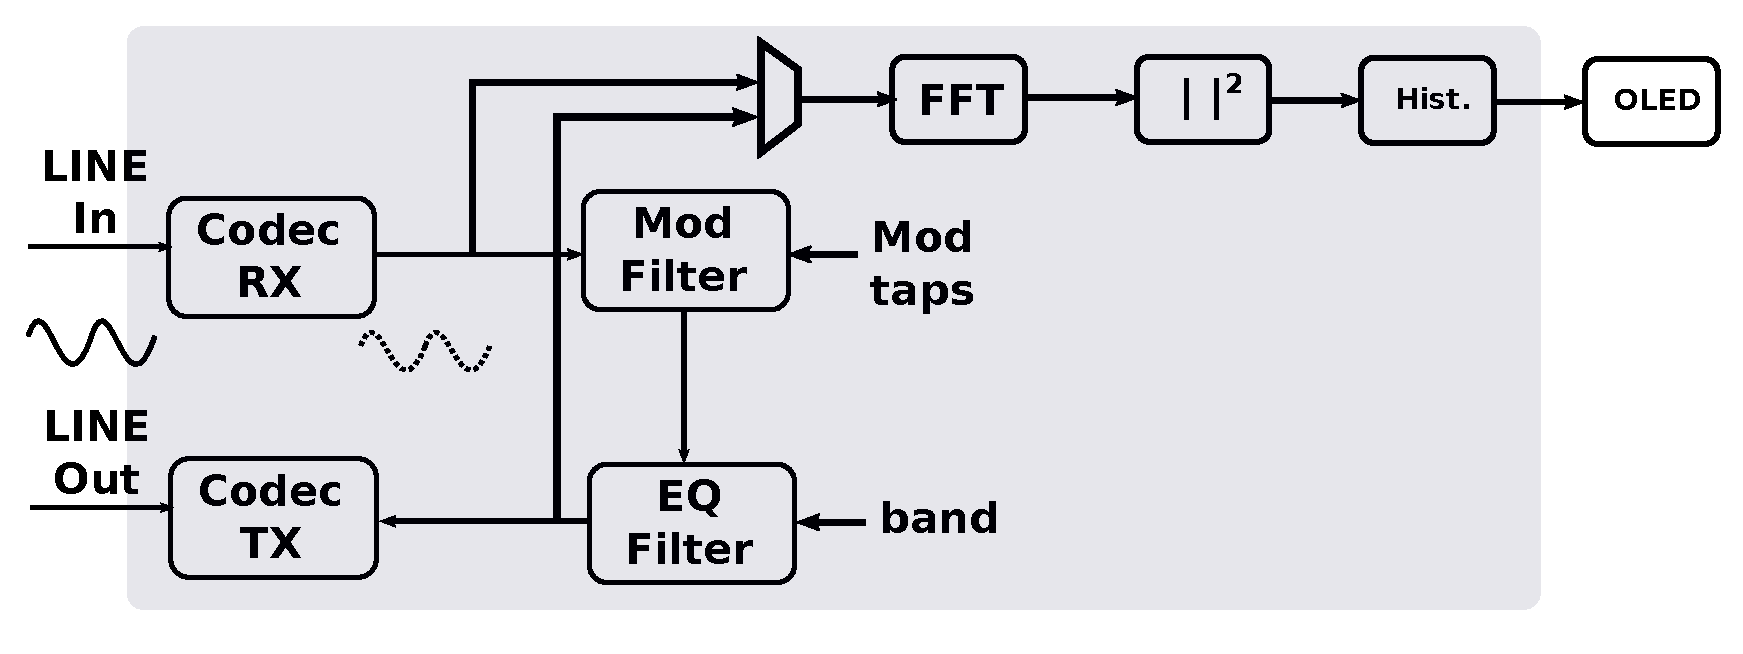
\includegraphics[width=0.75\linewidth]{bloc_design.pdf} \\
	Bloc design
\end{center}

All processing is real time and synchronous to the input
stream. The initial sample rate is 48 MHz, making the
input data rate 1.152 Gb/s. This is way more more than needed.
In this setup we would need gigantic FFT to reach a decent
resolution. We would also have to implement enormous filters
to obtain a meaningful output. \\

We use a CIC decimation filter with R = 128
to reduce the sample rate to 24 kHz (a little more than needed).
This reduces the bit rate to 576 kB/s. \\

One modulation can be applied on the signal,
as well as one EQ preset made of 16 subbands and
one Reverb/room profile can be emulated.
These are all implemented 
\& controlled in real time from the user interface.
For each step refer to its own documentation down below. \\

The modulation \& EQ will be applied using an FIR type
of implemntation. The Reverb profile will be implemented
by a 10 tap IIR type of filter. \\

A power spectral analysis is performed in real time,
either on the direct input line
or the final output line. Selection is done in
real time using the User Interface. Refer
to following section for further details.
The CIC decimator gives us a 187 Hz resolution in the spectral
analysis. The result is displayed in real time in the
form of a histogram, on the 'OLed' display. \\

By selecting either the direct input line
or the output line to feed the FFT, we
can choose to see the effect of the current filters
on the signal in spectral domain. \\

A final interpolation is obviously
needed to come back to the initial 1.152 Gb/s rate.

\newpage
\subsection{CIC filters}

CIC filters stand for Cascaode of Integrator and Comb Filters:
\begin{center}
	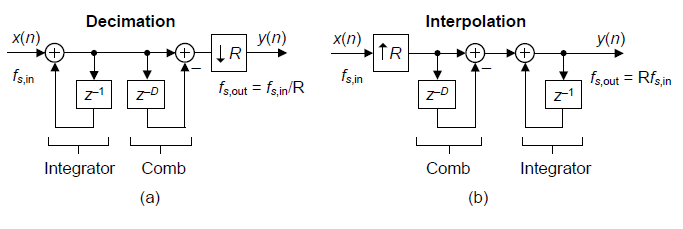
\includegraphics[width=0.75\linewidth]{CIC_digital_filters_fig6.png} \\
\end{center}

They are defined by 3 parameters:
\begin{itemize}
	\item R: decimation/interpolation factor
	\item M: time delay, can either be 1 or 2 cycle
	\item N: number of both integration \& comb stages
\end{itemize}

An integrator is defined by $H(z) = \frac{1}{1 - z^{-1}}$.
A comb filter is defined by $H(z) = 1 - z^{-M}$. \\

The total CIC filter is therefore defined by 
\begin{equation}
	H(z) = \left| \frac{1 - z^{-M}}{1 - z^{-1}} \right|^N
\end{equation}

The total filter gain is $(RM)^N$,
hence the total bit growth in our implementation
will be $\left[ log_2\left(RM^N\right) \right]_\text{ceil}$.
It is very important to take into account the bit growth, at least in the
itegrators. Ideally itegrators should implement a 2's complement format
with saturation, this is how our IP operates. \\

It is possible to approximate the magnitude response 
of a CIC filter to
$H(\nu) = \left| \frac{\sin(R M \pi \nu)}{R M \sin(\pi \nu)} \right|^N$
$\forall \nu$ normalized frequency. 
Hence the magnitude response has a $\frac{\sin(\nu)}{\nu}$ shape:

\begin{center}
	\begin{minipage}{0.40\linewidth}
		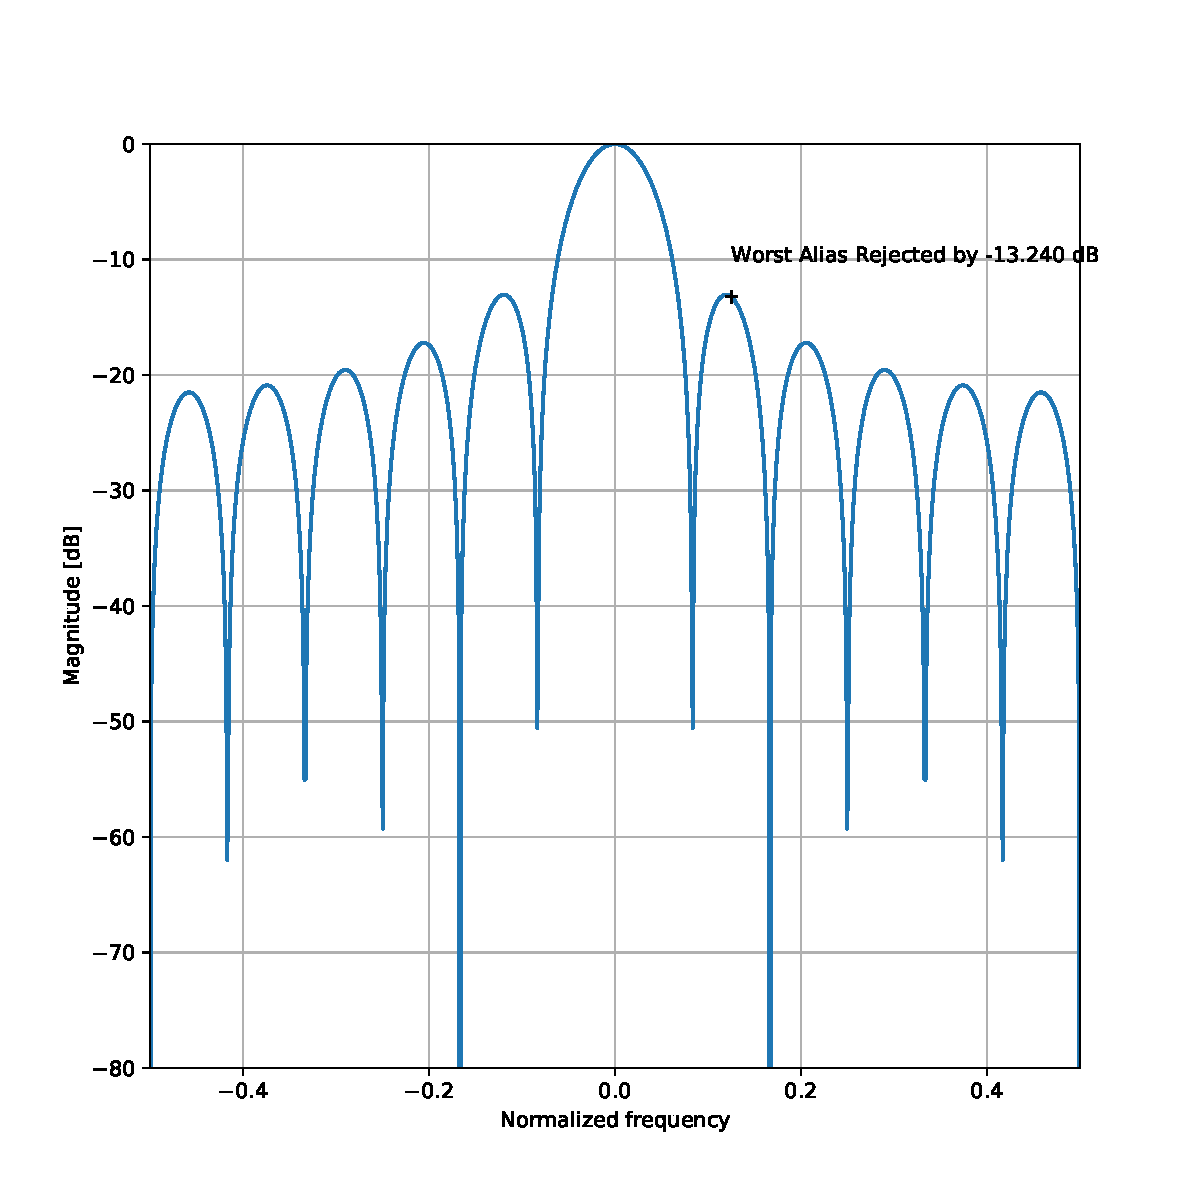
\includegraphics[width=0.99\linewidth]{cic_r12_n2.pdf} \\
		{\tt \$git/python/dsp/cic.py R=12 N=2} \\
		the worst alias is rejected by -13 dB
	\end{minipage}
	\begin{minipage}{0.40\linewidth}
		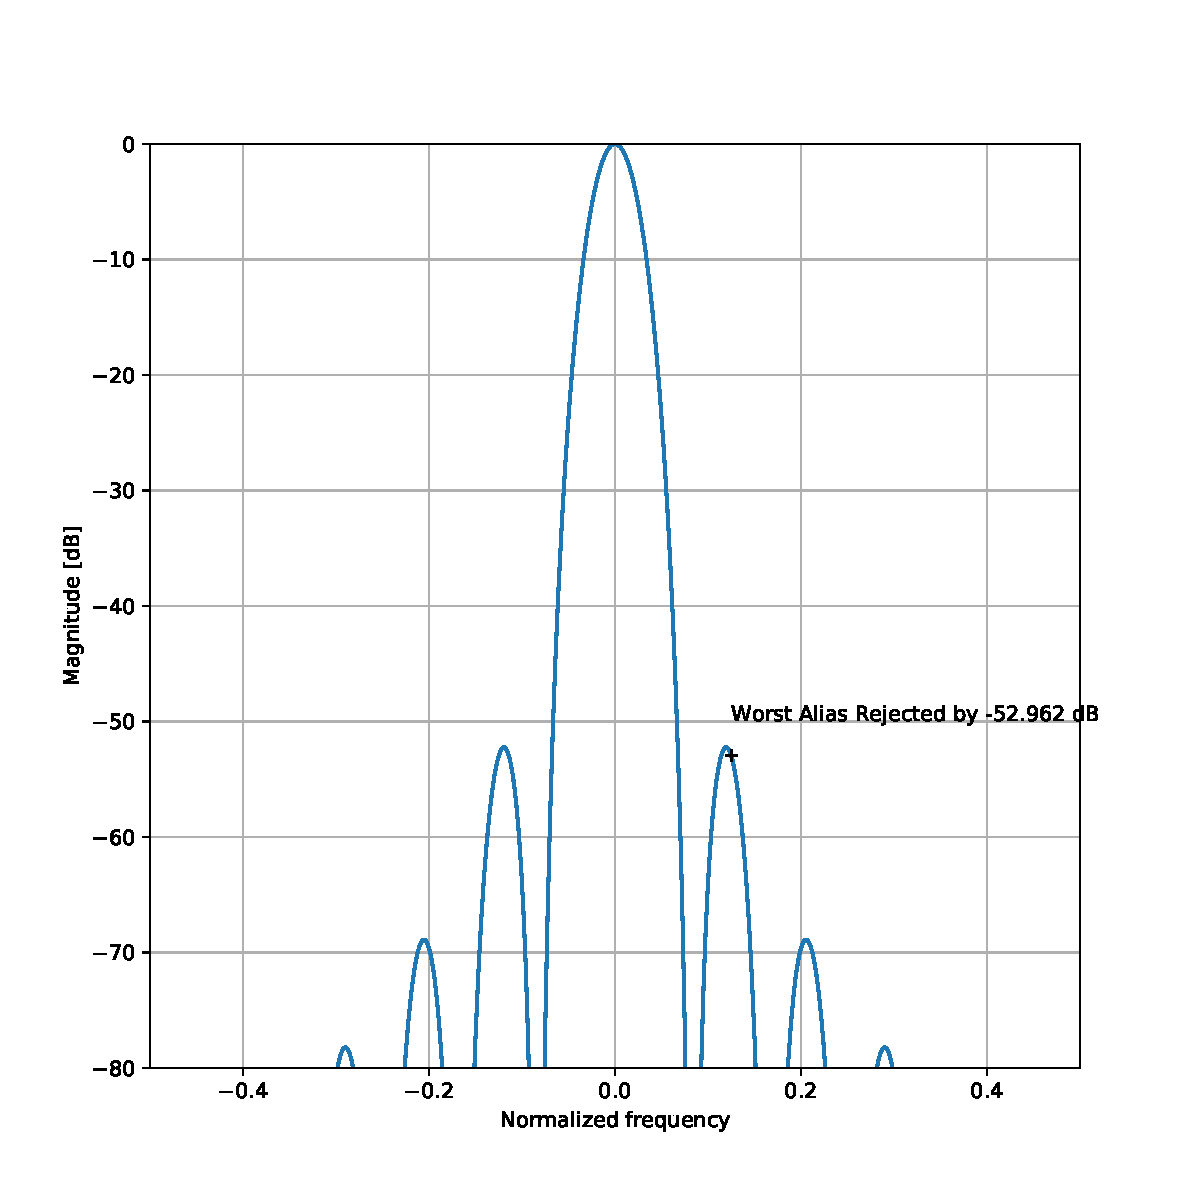
\includegraphics[width=0.99\linewidth]{cic_r12_n8.pdf} \\
		{\tt \$git/python/dsp/cic.py R=12 N=8} \\
		increasing the number of stages to 8
		improves the worst alias rejection to -53 dB
	\end{minipage}
\end{center}

The worst alias is encountered at the peak
of the 2nd lobe of the $\frac{\sin(\nu)}{\nu}$ shape, 
located at frequency $\nu = \frac{3}{2MR}$ \\

Because of this $f(\nu) = \frac{sin(\nu)}{\nu}$ shape,
we completely lose the flatness within the system
bandwidth. The transition bandwidth is also very slow.
To compensate for the flatness loss and to reduce
the transition, 
we generally use a compensation filter (in the form of an FIR
filter) after the CIC decimation filter
and prior the CIC interpolation filter. \\

In our system we will fix R=128 to reduce
the sample rate to 24 kHz and making our application
possible. We will see in the next section
how to design the compensation filter for this given
CIC filter.

\subsection{CIC compensation filter}

The compensation filter response is the exact inverse
of the CIC filter response $G(\nu) = \frac{1}{H(\nu)}$ 
within the new established band, ranging
from 0 to $\frac{f_s}{R}$,
$\frac{f_s}{R}$ being the first null of the $\frac{sin(\nu)}{\nu}$ response. \\

The CIC compensation filter is designed
using the python script {\tt \$git/dsp/cic-compensator.py}. 

\begin{verbatim}
   $git/dsp/cic-compensator.py R=4 N=12 BW=30
   $git/dsp/cic-compensator.py R=8 N=4 BW=45 ncoef=128
\end{verbatim}

Use BW (in \%) to set the pass band edge
location within the new established Nyquist band.
The ncoef parameter allows to compare different
implementation of the FIR filter.

\begin{center}
	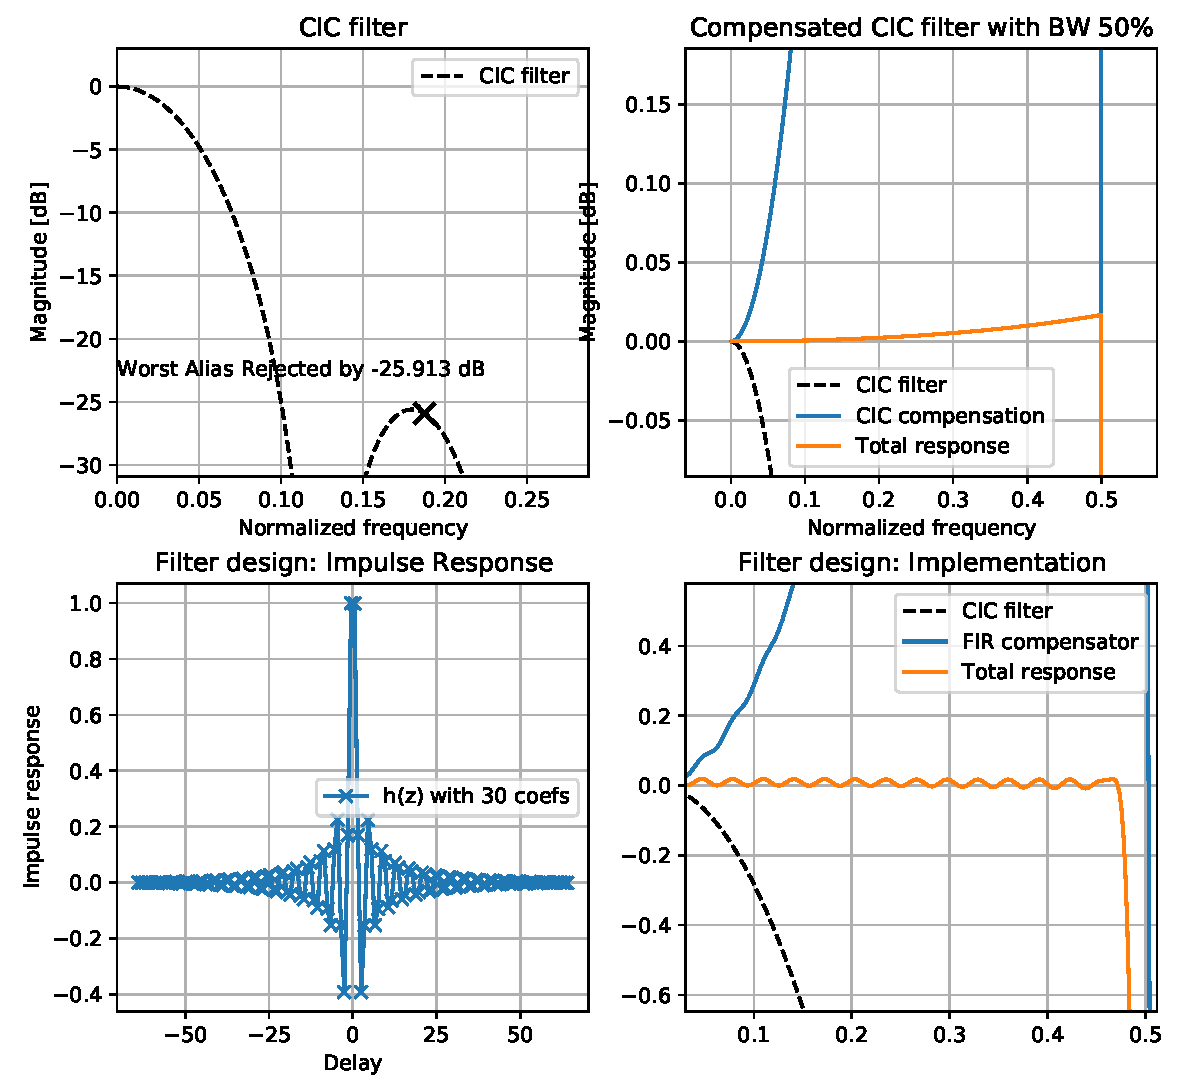
\includegraphics[width=0.75\linewidth]{fir-des-2.pdf} \\
	The CIC filter compensator designer designs a CIC
	filter to compensate for the CIC filtering stage.
	One can compare the effect of the BW cut off frequency
	(design the new user bandwidth) and the ripple effect,
	for different FIR filters implementation.
\end{center}

Upper left: theoretical CIC filter as described in previous
section. \\

Upper right: theoretical CIC filter versus its optimum
compensation, for a given BW parameter.
Total theoretical response is CIC+FIR. \\

Below - left: designed Impulse Response to be implemented,
for given BW and ncoef parameters. \\

Below - right: filter implementation: theoretical
CIC filter compensated by implemented FIR filter.
Total implemented response is CIC+FIR. \\

CIC filter compensation 
will be implemented in both the decimation
\& the interpolation filter, using
Xilinx's optimized FIR filter IP core. \\

The CIC decimation is very important
to our system, without heavily downsampling
the input signal (we chose R=128),
the displayed FFT resolution would be
37.5 MHz, which is totaly unusable for audio data.
The Modulation Filter \& EQ filter would require so 
many bands to be computated that it would also be impossible
to implement them in the system.

\begin{center}
	\begin{minipage}{0.40\linewidth}
		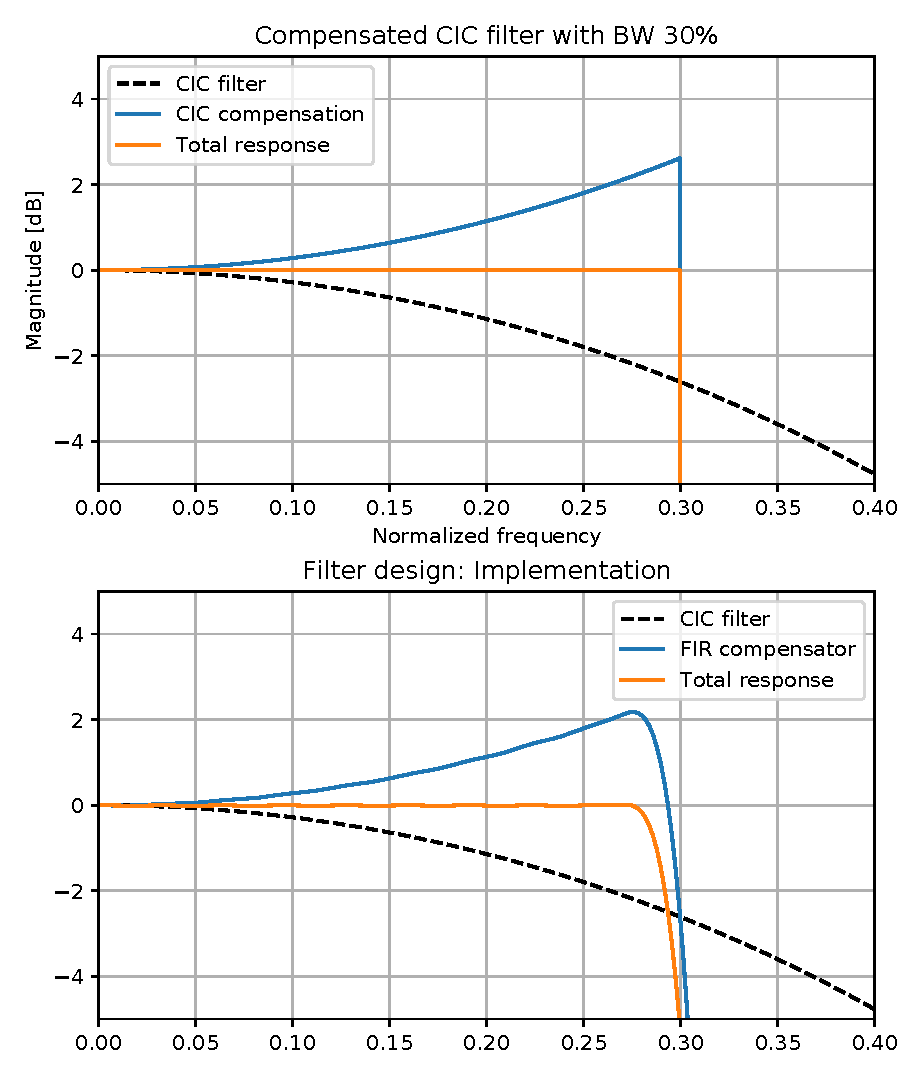
\includegraphics[width=0.99\linewidth]{fir-des-3.pdf}
		Direct cut off is impossible to reach in the implemented
		form. This is a 16 tap FIR filter.
	\end{minipage}
	\begin{minipage}{0.40\linewidth}
		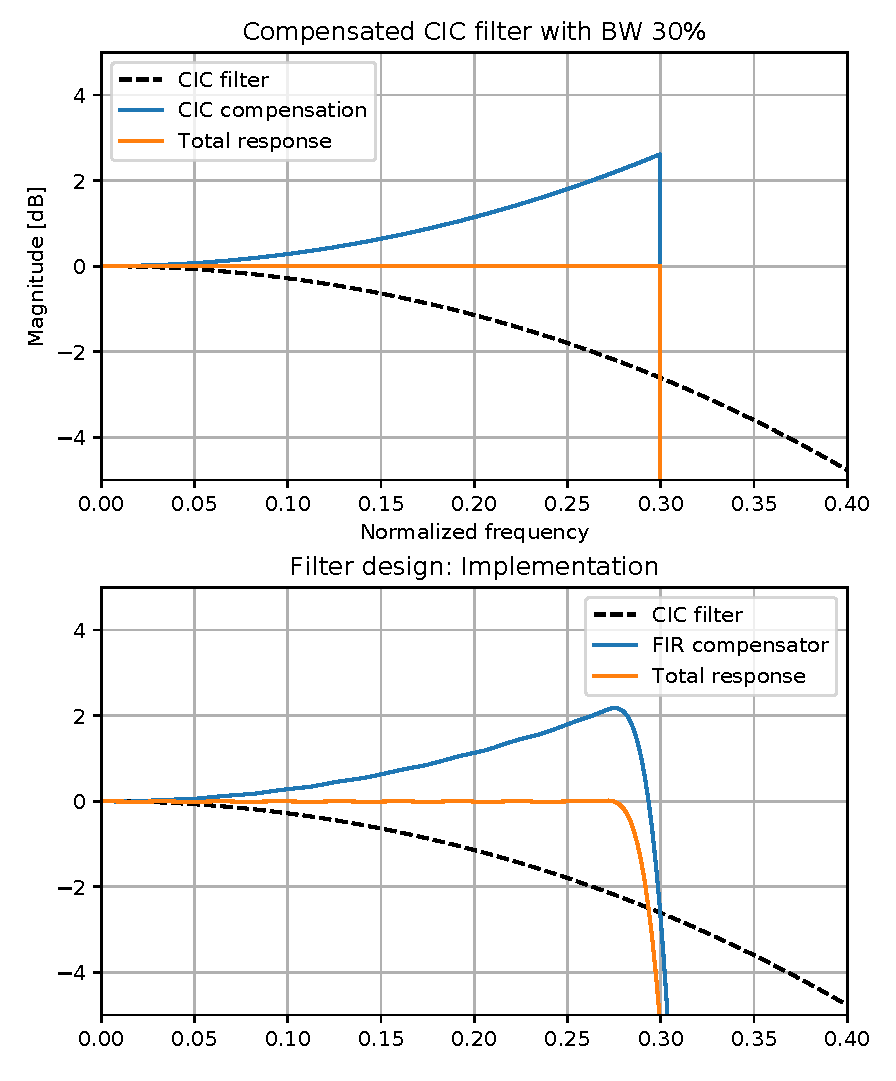
\includegraphics[width=0.99\linewidth]{fir-des-4.pdf}
		Increasing to 128 taps dramatically reduces
		the distortion within the band.
	\end{minipage}
\end{center}

\subsubsection{CIC interpolation filter}

Using previously designed compensated CIC decimator,
we reduce the input rate by a factor of 128.
We need to interpolate by a factor of 128 prior
outputing the signal to the DAC.


\newpage
\subsection{Equalization filter}

The EQ filter allows the user 
to modify the signal's frequency response,
in real time. \\

The frequency response is divided into 16 bands,
considering our internal sample rate of 
$f_s = \frac{48e8}{128} = 24$ kHz,
each band is 1.5 kHz wide. \\

The user interface allows the user
to define the weighting of each band,
so define the custom frequency response
$H(\nu)$. \\

The GUI transforms $H(\nu)$ into $h(z)$
to be applied in the FIR filter:

\begin{equation}
	\begin{split}
	h(z) = FFT^{-1}\left(H(z)\right) = Bilienear(H(\nu))
	\end{split}
\end{equation}

\newpage
\subsection{FFT Histogram}

The Histogram IP core converts
the power spectrum from the
magnitude IP core
to a histogram to be displayed on the OLED. \\

It is a simple mapping of the resulting
power spectrum to a 2D array (X,Y) describing
the power spectrum along a frequency axis. \\ 

%\begin{center}
%	\includegraphics[width=0.75\linewidth]{fft_histogram.pdf} \\
%\end{center}

\newpage
\section{Simulation}
\subsection{GHDL}

Most IPs are simple unitary functions
and can be simulated using {\tt ghdl}.
Any IP that comes with a {\tt /sim/Makefile}
can be simulated with {\tt ghdl}.

Install {\tt ghdl} to easily
simulate modules that come with a testbench:

\begin{verbatim}
git clone https://github.com/ghdl/ghdl
cd ghdl
./configure
make
sudo make install
\end{verbatim}

Once this is done, you can safely simulate a module
that comes with a testbench by using {\it make}
in its {\tt sim} folder.
For example:

\begin{verbatim}
cd $git/ip/adau1761/sim/rx
make
\end{verbatim}

\begin{center}
	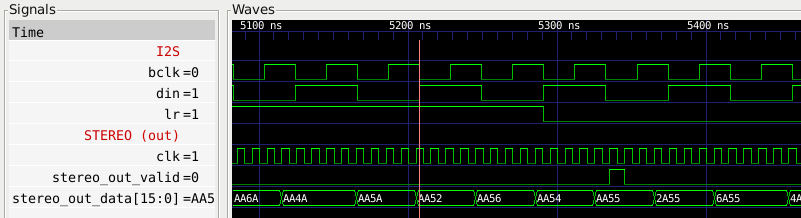
\includegraphics[width=0.75\linewidth]{ghdl-gtkw.png} \\
	{\tt GHDL} \& {\tt GTK-wave} are convenient
	tools to quickly run a simulation on a unitary IP
\end{center}

\subsection{Vivado - {\tt xsim}}

IPs that require Xilinx's dedicated functions,
such as BRAM or FIFOs to buffer the input/output
data, can only be simulated in Vivado.

To simulate those IPs on your side, either
import the IP sources \& dependencies and the testbench
into Vivado, or use the {\tt sim-project.tcl} if
it is delivered with the IP.

\end{document}
